As previously mentioned, we want to extend the work done by Ikenmeyer et al. \cite{ikenmeyer_WhatWhatNot_2022},
in order to analyse the combinatorial nature of \textbf{PPAD} as a whole.  Although the project
did not manage to achieve the desired theorem, we hope to demonstrate interesting findings that can allow
us to reveal more intricate properties of $\textbf{\#PPAD}$. Our first step is to extend the hierarchy
between \textit{EndOfLine} and \textit{SourceOrExcess}$(2,1)$. We can observe that
$$
\forall a,b \in \mathbb{N}: a \leq b \implies \textbf{\#PPAD}(\textit{SourceOrExcess})(a,1) \subseteq
\textbf{\#PPAD}(\textit{SourceOrExcess})(b,1)
$$
In fact, we can extend the degree of graphs to polynomial degrees.
For that we provide a formal definiton of the \textit{Unbalanced} problem \ref{def:unbalanced}


\begin{definitionbox}{\textit{Unbalanced} problem definition}{unbalanced}
    \textbf{Input}: We are given tuple $(\textbf{S}, \textbf{P}, f, g)$, such that
    $\mathbf{S} = \{S_i\}_{i \in [f(n)]}$ and $\mathbf{P} = \{P_i\}_{i \in [g(n)]}$ and
    $f,g: \mathbb{N} \to \mathbb{N}$ are poly-time computable polynomial functions.
    This describes a graph $G = (V, E)$ such that $V = \{0,1\}^n$ and
    $$
        \forall (x,y) \in E, \exists i \in [f(n)],j \in [g(n)] : S_i(x) = P_j(y)
    $$
    We enforce the condition that $\forall P_i: P_i(0^n) = 0^n$ and $\exists S_j: S_j(0^n) \neq 0^n$\\
    \textbf{Output}: A node $v \in \{0,1\}^n \smallsetminus \{0^n\}$ such that $\textit{in-deg}(v) \neq \textit{out-deg}(v)$. \\
    If $f(\cdot) = p$ or  $g(\cdot) = k$ for some $p, k \in \mathbb{N}$, we will denote the problem as $\textit{Unbalanced}(p, k)$
\end{definitionbox}


\begin{lemmabox}{}{unbalanced-lem-ppad-complete}
    \label{lem:unbalanced-lem-ppad-complete}
    $\textit{Unbalanced}$ is \textbf{PPAD}-complete \cite{hollender_ComplexityMultisourceVariants_2018}
\end{lemmabox}

As previously mentioned, Hollender et al. \cite{hollender_ComplexityMultisourceVariants_2018},
demonstrated how extending the number of known sources of the \textit{EndOfLine} problem
does not affect its \textbf{PPAD}-completeness. Moreover,
combinatorially we can observe that if a \textit{EndOfLine}
problem has $k$ known sources, it implies that there must exist $k$
at least $k$ solutions. This raises an interesting question as to
what happens when we combine the number of known sources of a graph with its degree.
For starters, we can observe that by lemma \ref{lem:unbalanced-lem-ppad-complete-sources},
the \textit{Unbalanced} problem is not affected.

\begin{lemmabox}{}{unbalanced-lem-ppad-complete-sources}
    $$
        \textbf{\#PPAD}(\textit{PolyS-Unbalanced}) \subseteq \textbf{\#PPAD}(\textit{Unbalanced})
    $$
\end{lemmabox}

\begin{proof}
    To show our reduction, that we have an instance of \textit{PolyS-Unbalanced},
    where have $f(n)$ known sources. Assume that $g(n)$ describes the input
    degree and $h(n)$ the output degree. We create a new \textit{Unbalanced}
    instance with in- and out-degree polynomials $p(n)= (\max\{g(n), h(n)\}) \cdot f(n)$.
    We will use the figure \ref{fig:unbalanced-ms-trans} to illustrate our reduction. Essentially, we are

    where $s_i$ is the $i$th known source of the original problem. For each node
    $k$ of the $i$th group, denoted as $v^i_k$, we are adding edge $v^i_k \to s_i$.
    Since each $s_i$ element has  $\textit{in-degree} = \textit{out-degree}$, we can
    observe that we are not creating any additional solutions. Since this transformation
    is local, any other unbalanced node will stay the same and therefore the set of Solutions
    is preserved.



    \begin{figure}[h!]
        \centering
        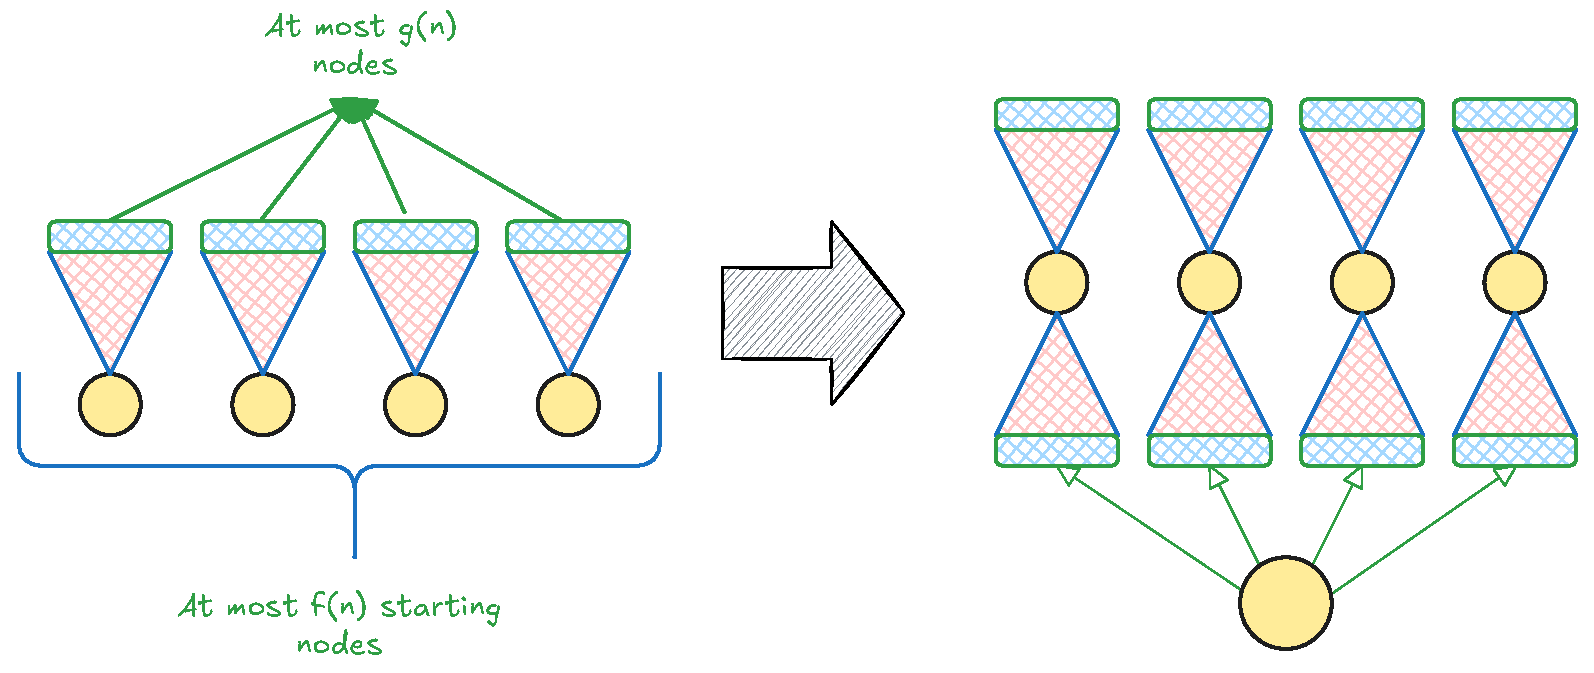
\includegraphics[width=0.5\textwidth]{Chapter3/unbalanced-multi-source.pdf}
        \caption{\textit{PolyS-Unbalanced} transformation to \textit{Unbalanced}}
        \label{fig:unbalanced-ms-trans}
    \end{figure}
\end{proof}

For simpler instances, such as the \textit{EndOfLine}, the reduction
demonstrated by Hollender is non parsimonious, meaning there is a
possibilitiy of an oracle separation betwwen \textit{EndOfLine} and \textit{2S-EoL}.
In fact one can observe that we can create a 3D-matrix of problems such that
$$
    \forall i, j, k \in \mathbb{N} \cup \{\textit{Poly}\} : M_{i,j,k} = k\textit{S-Unbalanced(i,j)}
$$
Where $\omega$ denotes polynomial values. 
Morover, these hierarchies seem to reveal some hidden combinatorial structures in \textbf{PPAD} and in
\textbf{TFNP} as a whole. 
For example, one can demonstrated the following claim \ref{clm:sc-deg-src}

\begin{claimbox}{SourceOrExcess with fixed degrees and sources}{sc-deg-src}
    Given $\alpha, \beta \in \mathbb{N}$, the problem $\alpha\textit{S-SourceOrExcess}(\beta,1)$ will have at least
    $\mu = \lceil \alpha/\beta \rceil$ solutions.
\end{claimbox}

\begin{proof}
    Given $\alpha\textit{S-SourceOrExcess}(\beta,1)$, in order to find
    the minimum number of solutions, we can assume that we there are no other sources other than the first $\alpha$ nodes.
    We argue that the minimum number of solutions is $\mu = \lceil \alpha/\beta \rceil$ since we can create 
    $\mu$ sinks that connect to at most $\beta$ nodes each. We will refer to these
    graphs as sink graphs.

    We can demonstrate that any graph can be reduced to a sink graph.
    Our first observation is to convert every excess node to a sink node. To do that we can apply two simplification 
    phases:
    \begin{enumerate}
        \item Removal phase: Remove all paths between two excess nodes or between excess and sink nodes.
        We can observe that after this steps our graph only contains sources and sinks.
        \item Merging phase: If there are sinks with degrees $(a,0)$ and $(b,0)$ such that
        $a + b \leq \beta$ then we can merge the two to remove a solution. Keep repeating this process until
        no two sinks can be merged
    \end{enumerate}
    We can observe that any graph will simplify to a sink graph and therefore we will always have at least $\mu$ solutions.
\end{proof}
This implies there exists subclasses in \textbf{PPAD} which we can denote as $\textbf{PPAD}(k)$ where we have \textbf{PPAD} problems with at least $k$ solutions.
This may lead in future directions where we can ask about combinatorial interpretations of $\textbf{PPAD}(\alpha)-\beta$ for $\alpha \geq \beta$.

% Third reason would be to demonstrate that an important milestone for our conjecture is to establish
% the relation between \textit{Unbalanced} and \textit{PureCircuit}. By our
% lemmas \ref{lem:unbalanced-lem-ppad-complete}, \ref{lem:unbalanced-lem-ppad-complete-sources}, we can observe
% that every possible variant of input, output degree and known sources can be eventually reduced to \textit{Unbalanced}.
% In addition, the majority of problems in \textit{PPAD} are related with each other by some form of an unbalanced directed graph,
% due to their eventual reductions to the \textit{EndOfLine} problems. We emphasize that this does not imply that every \textbf{PPAD}
% problem can be parsimoniously reduced to the \textit{Unbalanced} problem, but more to indicate some heuristical argument
% as to why this might be an important problem to study.